%   File: Golfer.tex
% Author: Adam Leeper
%------------------------------------------------------------------------------
%\\[0.45pc]
\providecommand{\isolatedBuild}[1]{#1}% Fallback definition to build normally.
\isolatedBuild{
  \documentclass[11pt,letterpaper]{book}
  %\documentclass[11pt,letterpaper]{book}

% aleeper: I think these are needed for Paul's macros?
\usepackage{epsfig}
\usepackage{epstopdf}

%\makeatletter
%\typeout{The import path is \import@path}
%\makeatother

\usepackage{import}

\subimport{./}{packagesMitiguy.sty}
\subimport{./}{macrosMitiguy.tex}
\subimport{./}{PageStylesMitiguy.tex}
\subimport{./}{macrosLeeper.tex}
   % Found via TEXINPUTS environment variable.
  \isolatedBuildHeader{Rolling and Linkage Constraints}
                      {Rolling and Linkage Constraints}
}
%%%
%%%
%%%
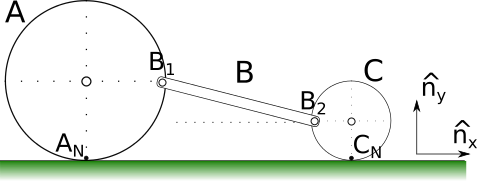
\includegraphics[width=12cm]{rolling_linkage.png}
\\[0.5pc]
The figure above shows wheels $A$ and $C$ connected by a link $B$.
Both wheels \textbf{roll} on the ground $N$. Let $\omega_A$, $\omega_B$,
and $\omega_C$ denote the $+\uvecz{n}$ (counter-clockwise) measures of angular
velocity of each body in $N$, respectively. Let the radius of the wheels be
$R_A$ and $R_C$, and the length of the linkage be $L_B$. Let $\theta$ be the
(acute) angle between $\uvecx{n}$ and the line connecting $B_1$ to $B_2$.
For the configuration shown:
%
\begin{enumerate}
  \item Calculate \vel{B_1}{N}, the velocity of point $B_1$ in $N$, in terms
    of $\omega_A$ and $R_A$.
    %
  \item Calculate \vel{B_2}{N}, the velocity of point $B_2$ in $N$, in terms
    of $\omega_C$ and $R_C$.
    %
  \item Using trig, find an expression for the (acute) angle $\theta$ in terms
    of $R_A$, $R_C$, and $L_B$.
    %
  \item Find a vector equation relating the velocity of $B_1$ and $B_2$.
    \textbf{Hint:} It is helpful to introduce a frame aligned with link B.
    %
  \item Set up a system of 2 scalar equations that would let you solve for
    $\omega_B$ and $\omega_C$.
    %
  \item Given that $w_A = 2$ rad/s, $r_A = 1$ m, $L_B = 2$ m, and $r_C = 0.5$ m,
    calculate values for $\omega_B$ and $\omega_C$.
\end{enumerate}
%
\isolatedBuildFooter